\documentclass{article}
\usepackage[a4paper, margin=0.75in]{geometry}
\usepackage{multicol}
\usepackage{tikz}
\usepackage{float}
\usepackage{graphicx}
\usetikzlibrary{shapes, arrows, positioning}
\title{FedCampus: Summer Research Report}
\author{
    Steven Hé (Sīchàng), Beilong Tang, Aicha Slaitane, Boyan Zhang,
    Tianjun Yuan\\
    Supervisor: Professor Bing Luo\quad
    Other mentor: Jiaqi Shao\\
    Supported by the DKU Office of UG Studies through the Summer Research
    Program.
}

\begin{document}
\maketitle

\begin{abstract}
The FedCampus project aims to establish a privacy-preserving data
platform for a smart DKU campus by integrating edge devices. We discuss
the development of an Android application (The App) that serves as a
first step in FedCampus. The App accesses users' health
data to facilitate Federated Learning (FL) and Federated Analytics (FA),
two Data Science research fields prioritizing data privacy. To power The
App, we developed a dedicated FL platform and constructed sleep
efficiency prediction ML models. To date, The App is in alpha testing
phase and we anticipate to launch it in the fall semester.
\end{abstract}


\setlength{\columnsep}{0.25in}
\begin{multicols}{2}
\section{Introduction}

The FedCampus project aims to create a privacy-preserving data platform
for a smart DKU campus, integrating edge devices like smartphones and
smartwatches. Central to FedCampus is the development of a system that
orchestrates data aggregation and analysis from edge devices, propelling
Federated Learning (FL) and Federated Analytics (FA).

FL and FA are two innovative Data Science research fields prioritizing
data privacy. FL trains Machine Learning (ML) models directly on edge
devices with localized data. FA analyzes dispersed data across devices
without central data consolidation.

In the initial phase of FedCampus, we aim to develop an Android
application (The App) to locally access users' health
data from Huawei HealthKit (HUAWEI Developers, n.d.) for FL and FA
functionalities. We would recruit volunteers on DKU campus to use The
App. It would train a sleep efficiency prediction ML model and generate
population statistics.

Sleep efficiency holds significance due to its impact on human
well-being, influencing factors like fatigue alleviation, improved work
performance, and overall health. Population statistics on health help
people understand their own health conditions and encourage them to
engage in improving it.

We will discuss three aspects of our work: FL workflow, ML model, and
The App.

\section{Methodology}

\subsection{Federated Learning (FL) Workflow}

In its FL workflow, FedCampus integrates established libraries and
standards strategically. We employ a backend constructed using Django
REST Framework (``Django REST framework: Home'', n.d.). For
orchestrating FL scheduling and model aggregation in the backend, we
leverage the full capabilities of Flower (``Flower: A Friendly Federated
Learning Framework'', n.d.), an open-source FL framework. Within The
App, we integrate TensorFlow Lite (``TensorFlow Lite'', n.d.) to
facilitate Android on-device ML training, and communicate with our
backend using Flutter (``Flutter'', n.d.) HTTP and gRPC (``gRPC'', n.d.)
libraries.

Our FL workflow includes the following three steps, as illustrated in Figure
\ref{fig:fl-workflow}:

\begin{enumerate}
\def\labelenumi{\arabic{enumi}.}
\item
  \begin{quote}
  Model Request: The App requests the backend for an ML model.
  \end{quote}
\item
  \begin{quote}
  Training Initiation: The App requests the backend to spawn a Flower
  server that trains with the ML model, initiating FL training.
  \end{quote}
\item
  \begin{quote}
  Training: The App connects to the Flower server and undertakes the FL
  training tasks. During training, The App sends telemetry information
  to the backend.
  \end{quote}
\end{enumerate}

\begin{figure}[H]
\centering
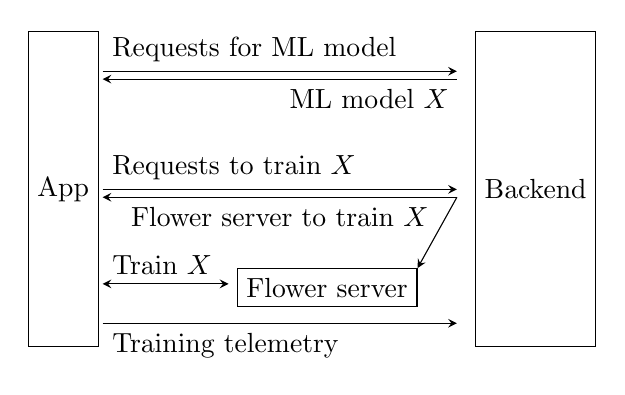
\begin{tikzpicture}
    \node[draw, minimum height=4cm] at (0, 0) {App};
    \node[draw, minimum height=4cm] at (6, 0) {Backend};
    \draw[-stealth] (0.5, 1.5) node[above right]{Requests for ML model} --
                    (5.0, 1.5);
    \draw[stealth-] (0.5, 1.4) -- node[below right]{ML model $X$}
                    (5.0, 1.4);
    \draw[-stealth] (0.5, 0.0) node[above right]{Requests to train $X$} --
                    (5.0, 0.0);
    \draw[stealth-] (0.5,-0.1) -- node[below]{Flower server to train $X$}
                    (5.0,-0.1);
    \draw[stealth-] (4.5,-1.0) node[below left, draw]{Flower server} --
                    (5.0,-0.1);
    \draw[stealth-stealth] (0.5,-1.2) node[above right]{Train $X$} --
                           (2.1,-1.2);
    \draw[-stealth] (0.5,-1.7) node[below right]{Training telemetry} --
                    (5.0,-1.7);
\end{tikzpicture}
\caption{FL workflow}
\label{fig:fl-workflow}
\end{figure}

\subsection{Sleep Efficiency ML Model}

With our ML model, we aim to predict how daily physical activities
influence same-day sleep efficiency and how past days'
activities impact next-day sleep efficiency for the DKU community. We
constructed these ML models using Tensorflow and Keras tuner and
pre-trained them using the PMDataset (``PMData: A Sports Logging
Dataset'' 2020), an open-source lifelogging dataset chronicling the
activities of 16 individuals over a five-month period.

\subsection{The App}

Constructed using Kotlin (``Kotlin Programming Language'', n.d.) native
code and the Flutter framework (``Flutter'', n.d.), the development of
The App showcases the applications of FL and FA.

The App retrieves health data from Huawei HealthKit (HUAWEI Developers,
n.d.) facilitated through wearable devices. These data are sleep
efficiency, step count, calories burned, intensity time, stress,
distance, and heart rate. This data acquisition process is enabled
through direct integration with Huawei HealthKit' s
Kotlin API. Health data are synchronized from wearable devices through
the Huawei HealthKit app to The App. For high and reliable performance,
The App strategically employs a local database to cache previously
fetched data. The acquired data undergoes formatting and cleaning
processes to ensure its accuracy and reliability.

As an FA functionality, The App employs the Differential Privacy (DP)
mechanism to generate statistics. Specifically, it adds random numbers
of normal distribution to the collected data before uploading them to
the server. The server then executes traditional statistical analysis
using these data with noise.

\section{Results}

\subsection{FedKit}

We developed FedKit, an open-source FL platform tailored for the needs
of The App. FedKit orchestrates our entire FL workflow. It includes a
backend server, an Android library for on-device training, and a Flutter
library for client-side communication.

FedKit is meticulously customized to address the requirements of
FedCampus. Its backend is designed for persistence, facilitating
on-demand FL training. The platform allows backend-oriented
interchangeability of ML models employed for FL training. The FedKit
client generates telemetry data about the training progress, empowering
comprehensive analysis of training performance.

\subsection{Sleep efficiency ML model}

We developed two sleep efficiency prediction models, for either same-day
or next-day prediction. Both models have high performance during
centralized pre-training.

\subsection{The FedCampus App (The App)}

The App is in alpha testing phase and will be launched in the fall
semester.

The App showcases FL through the training of our next-day sleep
efficiency prediction ML model using FedKit. Operating on a seven-day
health data interval, it periodically executes the training procedure in
the background once opened by the user, minimizing user interaction.
Incorporating DP, The App also demonstrates FA by showing the users the
average value of each health data metric and their ranking.

\begin{figure}[H]
\centering
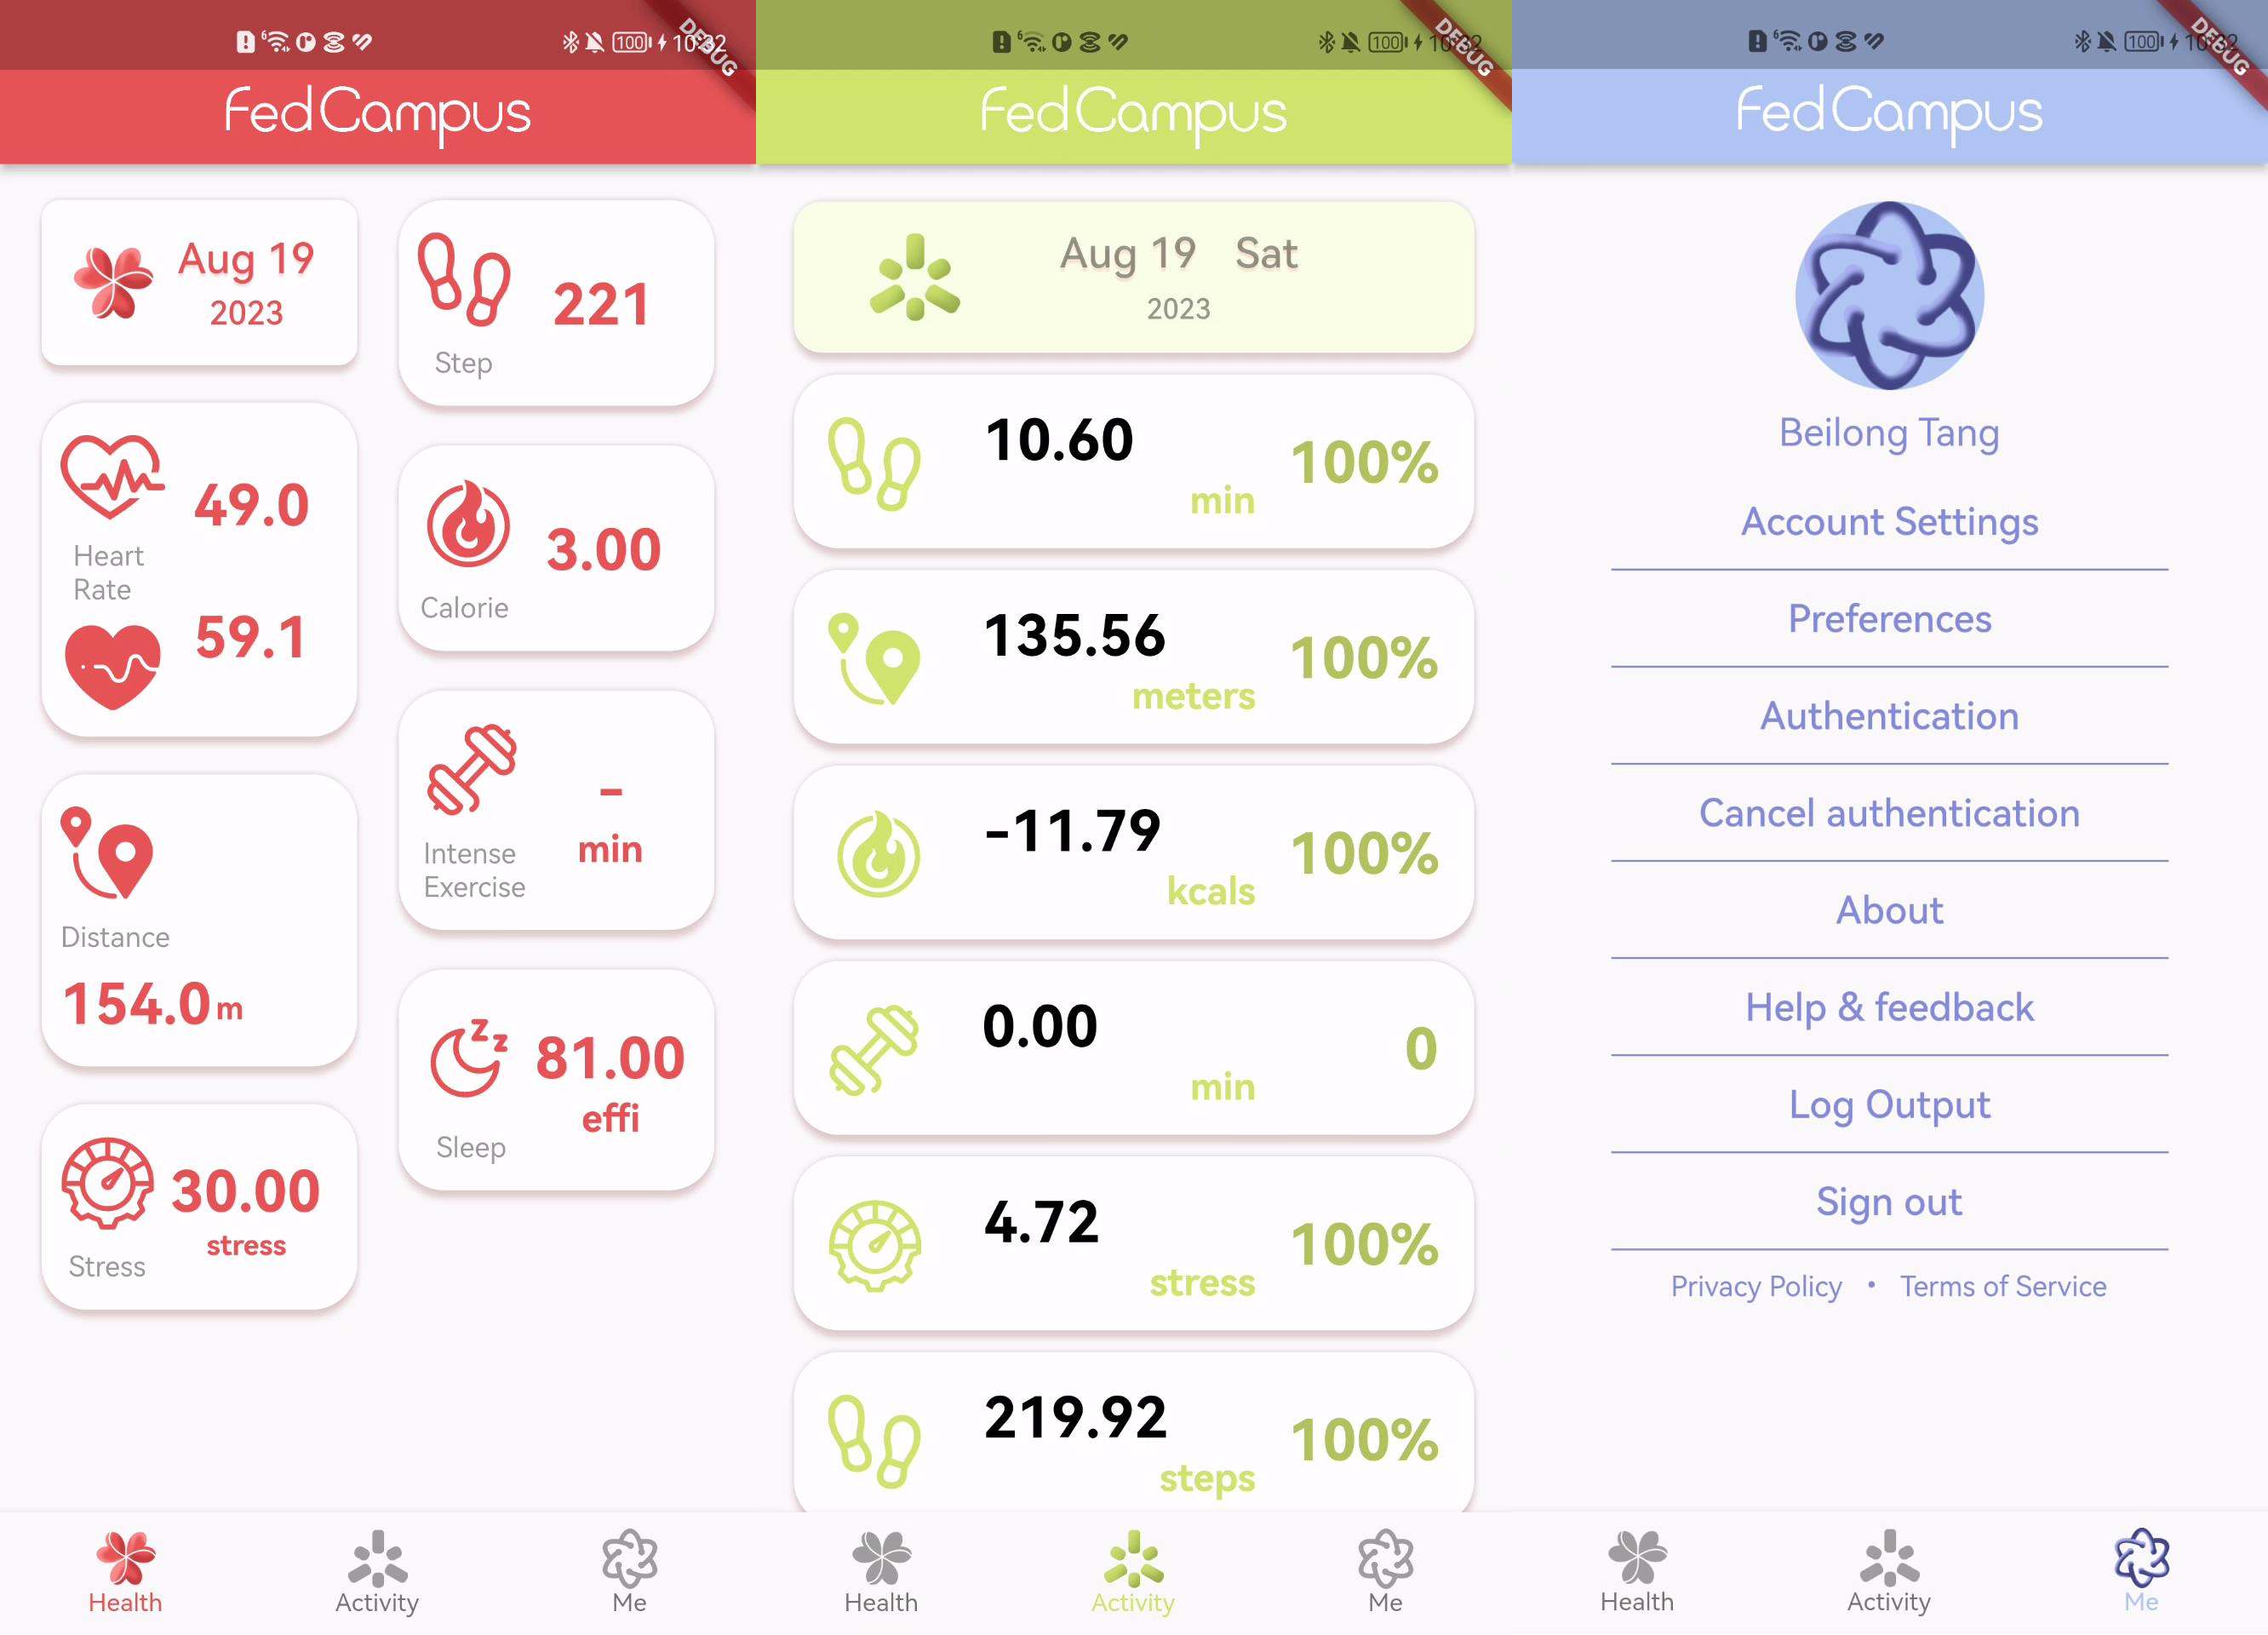
\includegraphics[scale=0.1]{fedcampus-app.jpg}
\caption{Health page in The FedCampus App}
\label{fig:app}
\end{figure}

\section{Conclusion}

The FedCampus project endeavors to establish an innovative
privacy-preserving data platform to integrate edge devices with FL and
FA. As a first step and demonstration of the project' s
concepts, the developed Android app is powered by the tailor-made FedKit
to train our sleep efficiency prediction model and generate DP
statistics. Looking ahead, the FedCampus project will extend its support
to the iOS ecosystem and data channels other than Huawei HealthKit,
driving towards an inclusive smart campus.

\section{Publication Plans}

We plan to submit our systems work to the AAAI-24 Demonstration Program.
If our paper is accepted, we will perform live demonstrations of our
work at the 38th Annual AAAI Conference on Artificial Intelligence.
\end{multicols}

\pagebreak
\section{References}
\begin{quote}

``Django REST framework: Home.'' n.d. Django REST framework: Home.
Accessed August 18, 2023. https://www.django-rest-framework.org/.

``Flower: A Friendly Federated Learning Framework.'' n.d. Flower: A
Friendly Federated Learning Framework. Accessed August 18, 2023.
https://flower.dev.

``Flutter.'' n.d. Flutter - Build apps for any screen. Accessed August
18, 2023. https://flutter.dev.

``gRPC.'' n.d. gRPC.io. Accessed August 18, 2023. https://grpc.io.

HUAWEI Developers. n.d. ``Health Kit - HUAWEI Health - HUAWEI
Developer.'' Huawei Developer. Accessed August 18, 2023.
https://developer.huawei.com/consumer/en/hms/huaweihealth/.

``Kotlin Programming Language.'' n.d. Kotlin Programming Language.
Accessed August 18, 2023. https://kotlinlang.org.

``PMData: A Sports Logging Dataset.'' 2020. OSF. https://osf.io/vx4bk/.

``TensorFlow Lite.'' n.d. TensorFlow. Accessed August 18, 2023.
https://www.tensorflow.org/lite.
\end{quote}
\end{document}
